% 
% Lecture Template for ME3023 -  Measurements in Mechanical Systems - Tennessee Technological University
%
% Spring 2020 - Summer 2020 - Fall 2020
% Tristan Hill, May 07, 2020 - June 12, 2020 - August 23, 2020
% Module 2 - To Err is Human
% Topic 2 - Errors and Uncertainty
% 
%

\documentclass{beamer}                         % for presentation (has nav buttons at bottom)
%\documentclass[handout]{beamer}  % for handout 
\usepackage{beamerthemesplit}
\usepackage{amsmath}
\usepackage{listings}
\usepackage{multicol}
\usepackage{framed}

\beamertemplateballitem 


\definecolor{TTUpurple}{rgb}{0.3098, 0.1607, 0.5176} % TTU Purple (primary)
\definecolor{TTUgold}{rgb}{1.0000, 0.8666, 0.0000} % TTU Gold (primary)

\setbeamercolor{palette primary}{bg=TTUpurple,fg=TTUgold}
\setbeamercolor{palette secondary}{bg=black,fg=TTUgold}
\setbeamercolor{palette tertiary}{bg=black,fg=TTUpurple}
\setbeamercolor{palette quaternary}{bg=TTUgold,fg=black}
\setbeamercolor{structure}{fg=TTUpurple} % itemize, enumerate, etc
\setbeamercolor{section in toc}{fg=TTUpurple} % TOC sections

% custom colors
\definecolor{TTUpurple}{rgb}{0.3098, 0.1607, 0.5176} % TTU Purple (primary)
\definecolor{TTUgold}{rgb}{1.0000, 0.8666, 0.0000} % TTU Gold (primary) 
\definecolor{mygray}{rgb}{.6, .6, .6}
\definecolor{mypurple}{rgb}{0.6,0.1961,0.8}
\definecolor{mybrown}{rgb}{0.5451,0.2706,0.0745}
\definecolor{mygreen}{rgb}{0, .39, 0}
\definecolor{mypink}{rgb}{0.9960, 0, 0.9960}

% color commands
\newcommand{\R}{\color{red}}
\newcommand{\B}{\color{blue}}
\newcommand{\BR}{\color{mybrown}}
\newcommand{\K}{\color{black}}
\newcommand{\G}{\color{mygreen}}
\newcommand{\PR}{\color{mypurple}}
\newcommand{\PN}{\color{mypink}}
\newcommand{\OR}{\color{TTU}}
\newcommand{\GD}{\color{TTUgold}}


\setbeamercolor{palette primary}{bg=TTUpurple,fg=TTUgold}
\setbeamercolor{palette secondary}{bg=black,fg=TTUgold}
\setbeamercolor{palette tertiary}{bg=black,fg=TTUpurple}
\setbeamercolor{palette quaternary}{bg=TTUgold,fg=black}
\setbeamercolor{structure}{fg=TTUpurple} % itemize, enumerate, etc
\setbeamercolor{section in toc}{fg=TTUpurple} % TOC sections

%\usefonttheme{professionalfonts}

\newcommand{\Lagr}{\mathcal{L}} % lagrangian

\newcommand{\hspcu}{\underline{\hspace{25mm}} } % large horizontal space w underline
\newcommand{\vspccc}{\vspace{6mm}\\} % large vertical space
\newcommand{\vspcc}{\vspace{4mm}\\}   % medium vertical space
\newcommand{\vspc}{\vspace{2mm}\\}     % small vertical space

\newcommand{\hspcccc}{\hspace{10mm}} % large horizontal space
\newcommand{\hspccc}{\hspace{6mm}} % large horizontal space
\newcommand{\hspcc}{\hspace{4mm}}   % medium horizontal space
\newcommand{\hspc}{\hspace{2mm}}     % small horizontal space

\newcommand{\eqscl}{0. 9}     % small horizontal space


\author{ME3023 - Measurements in Mechanical Systems} % original formatting from Mike Renfro, September 21, 2004

\newcommand{\MNUM}{2\hspace{2mm}} % Module number
\newcommand{\TNUM}{2\hspace{2mm}} % Topic number 
\newcommand{\moduletitle}{To Err is Human}
\newcommand{\topictitle}{Errors and Uncertainty} 

\newcommand{\sectiontitleI}{Random and Systematic Errors}
\newcommand{\sectiontitleII}{Dart Board Example}
\newcommand{\sectiontitleIII}{Types of Errors}
\newcommand{\sectiontitleIV}{Sample Uncertainty Data}

% custom box
\newsavebox{\mybox}

\title{Module \MNUM - \moduletitle}

\date{Mechanical Engineering\vspc Tennessee Technological University}

\begin{document}

\lstset{language=MATLAB,basicstyle=\ttfamily\small,showstringspaces=false}

\frame{\titlepage \center\begin{framed}\Large \textbf{Topic \TNUM - \topictitle}\end{framed} \vspace{5mm}}

% Section 0: Outline
\frame{

\large \textbf{Topic \TNUM - \topictitle} \vspace{3mm}\\

\begin{itemize}

	\item \sectiontitleI		\vspc % Section I
	\item \sectiontitleII 	\vspc % Section II
	\item \sectiontitleIII 	\vspc %Section III
	\item \sectiontitleIV 	\vspc %Section IV

\end{itemize}

}

% Section 1
\section{\sectiontitleI}

\frame{
\frametitle{\sectiontitleI}

``Errors are effects that cause a  measured value to differ from its true value. \hspcu error causes a
\hspcu variation in measured values found during repeated measurements of a variable. \vspc
\hspcu error causes an offset between the mean value of the data set and its true value. Both \hspcu and
\hspcu errors affect a system’s accuracy.''

\vspace{10mm}
{\tiny Text: Theory and Design of Mech. Meas.}
}
% Section 2
\section{\sectiontitleII}

\frame{
\frametitle{\sectiontitleII}

``The concept of accuracy and the effects of {\PR systematic} and {\PN random} errors in instruments
and measurement systems can be illustrated by the throw of darts.''

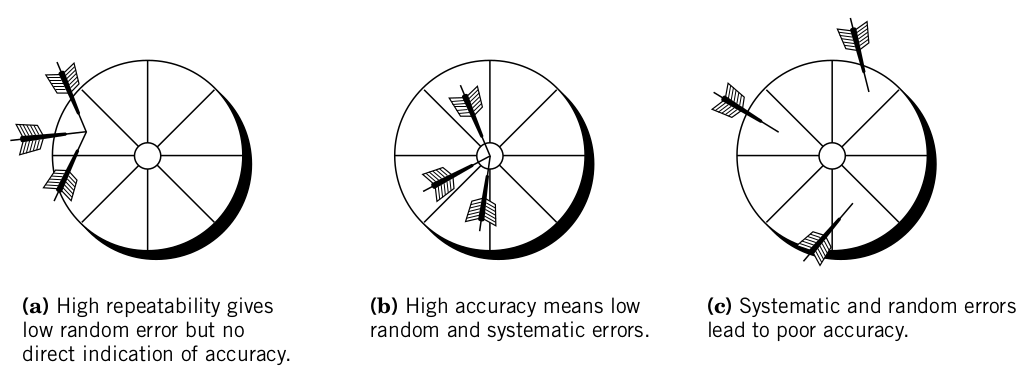
\includegraphics[scale=.20]{dart_throw.png}

``The ability of a measurement system to indicate the same value on repeated but independent
application of the same input provides a measure of the instrument \hspcu.''

{\tiny Text, Image: Theory and Design of Mech. Meas.}
}


% Section 3
\section{\sectiontitleIII}

\frame{
\frametitle{\sectiontitleIII}

Common categories of errors in measurements are shown below. This is not an exhaustive list.  

\begin{itemize}
	
	\item Linearity Error \vspc
	\item Sensitivity \vspc
	\item Zero (offset) Error \vspc
	\item Hysteresis Error \vspc
	\item Overall Instrument Error \vspc
\end{itemize}

\scalebox{1}{$u_c=\sqrt{u_1^2+u_2^2+...+u_M^2}$}


}

% Section 4
\section{\sectiontitleIV}

\frame{
\frametitle{Sample Uncertainty Data}

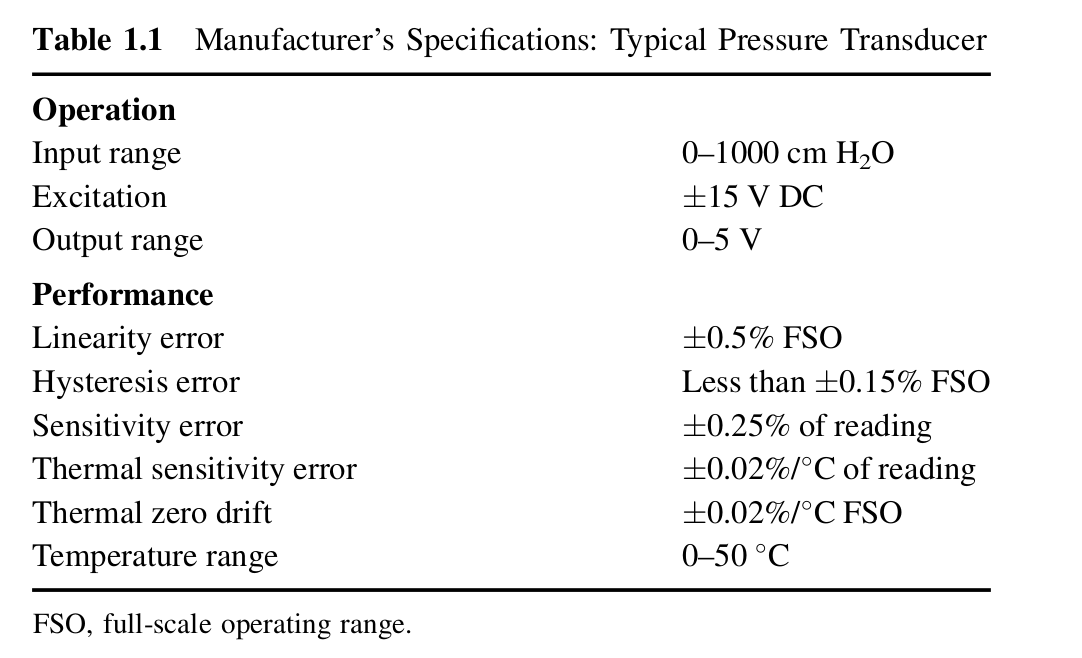
\includegraphics[scale=.22]{sample_uncertainties.png}

{\tiny Text, Image, Data: Theory and Design of Mech. Meas.}
}
\end{document}





